% !TEX root = Tesi.tex
\chead{}
\chapter{The combined approach}

\section{The IFML language}

The Interaction Flow Modeling Language (IFML)\cite{IFML-1, IFML-2} is designed for describing and controlling the behavior of front-end software applications, it brings several advantages to the development process such as promoting the separation of concerns between roles and increasing the overall understanding of the product for non-technical stakeholders. To achieve so IFML supports formal specification for interface composition, user interaction and event management independently of the implementation platform and it was adopted as a standard by the Object Management Group (OMG) in March 2013.

IFML supports the following concepts: 

\begin{itemize}
  \item \textbf{The view structure} describes \textit{ViewContainers}, their nesting relationships, their visibility and their reachability.
    
  \item \textbf{The view content} manages \textit{ViewComponents}, i.e., content and data entry elements contained within ViewContainers.
  
  \item \textbf{The events} defines the \textit{Events} that may affect the state of the user interface. \textit{Events} can be produced by the user’s interaction, by the application, or by an external system; 

  \item \textbf{The actions} triggered by the user’s events. The effect of an \textit{Event} is represented by an \textit{InteractionFlow} connection, which connects the event to the \textit{ViewContainer} or \textit{ViewComponent} affected by the \textit{Event}. The \textit{InteractionFlow} expresses a change of state of the user interface: the occurrence of the event triggers a change in the state that produces a transition in the user interface.
  
  \item \textbf{The navigation flow} indicates the effect of an Event on the user interface and represents an input-output depencency, the source of the input has some output that is associated with the input of the target of the link.

  \item \textbf{The data flow} indicates the data passed between \textit{ViewComponents} and \textit{Actions}
  
  \item \textbf{The parameter binding} illustrates the input-output dependencies between \textit{ViewComponents} and between \textit{ViewComponents} and \textit{Actions}. 


\end{itemize} 

\vspace{0.5cm}
\begin{figure}[htbp]
  \centering
    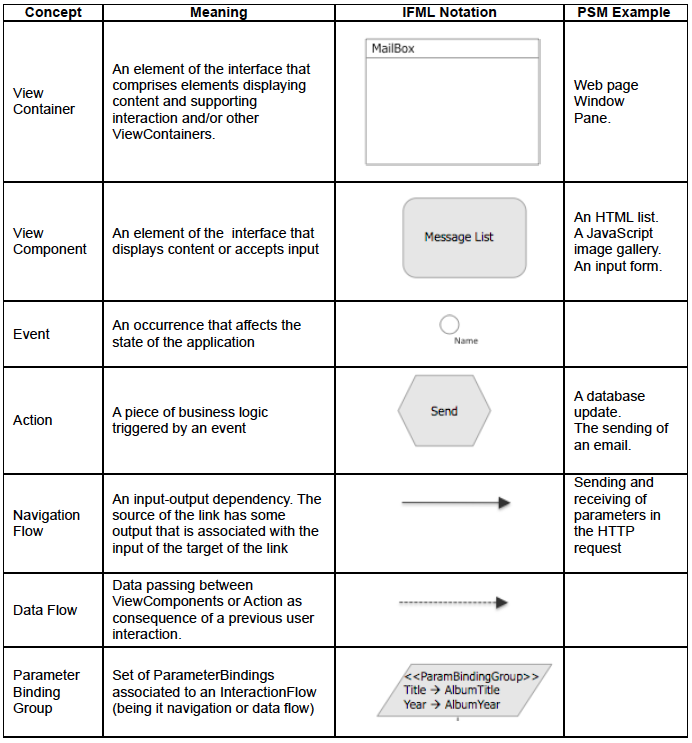
\includegraphics[height=10cm]{images/ifml.jpg}
  \caption{Main IFML concepts and notations.}
  \label{fig:ifml}
\end{figure}
\vspace{0.5cm}

\section{User interaction modeling for an eCommerce website}

eCommerce website front ends are usually built using shared and reusable components (forms, list views, detail views, etc.) which have a specific and expected behavior.
For example, Product lists and grids show record details for the user to view and interact with an action on these, call to action "Add To Cart" buttons are instead presented within product pages to trigger a different response and so on.
All these interactive operations can be represented using the IFML notation. 









\section{Pattern recognition}



